\section{Experiment 10D: learned compatible groups with unknown cardinality}
\label{sec:experiment10d}

\paragraph{Question and hypothesis.}
Experiment 10B established the value of complementary coverage when the
physical family of every client is supplied to the estimator. That oracle
partition is not a credible deployment assumption. Experiment 10D therefore
asks whether clients can be grouped from their restricted local records, while
also selecting the number of groups, and still retain the cold-start benefit
of family sharing. The intended claim is deliberately task based: the method
must discover clients that can share an LPV backbone, not reconstruct the
simulator's physical labels.

\paragraph{Protocol.}
The experiment uses ten new 30-client fleets (seeds 361--370), the nonlinear
tanh-tire plant, and the order-seven basis frozen in Experiment 10A. Each
client observes one contiguous block of the 10--30~m/s grid: three speeds in
the first three blocks and two in the final block. At every observed speed,
36 noisy perturbation transitions are used to estimate the six entries of the
local discrete-time state/input matrix. Blocks are stratified within physical
families solely to keep the simulated information-coverage comparison
balanced. The learned estimator receives neither those family labels nor the
oracle partition.

Fitting order-seven models independently before clustering would be invalid:
every local scheduling block is rank deficient by construction. We instead fit
a hard mixture of LPV regressions directly to the observed speed--matrix pairs.
For a candidate group count $K$, initialization uses $K$-means on each
client's mean residual relative to the global LPV fit. The algorithm alternates
between fitting one pooled LPV regression per group and assigning every client
to the model with the smallest variance-normalized residual on its own record.
We use 12 deterministic restarts, require at least five clients per group, and
consider $K\in\{1,\ldots,5\}$. The selected count minimizes
\begin{equation}
 \mathrm{BIC}_K=N\log(\mathrm{SSE}_K/N)
 +(42K+K-1)\log N,
\end{equation}
where $N$ is the number of scalar matrix observations, 42 is the coefficient
count of one six-output order-seven LPV map, and SSE is computed after scaling
each matrix entry by its across-client observation standard deviation.

\paragraph{Comparators and gates.}
LearnedCluster is compared with the restricted Local model, one Global LPV
model, OracleFamily, the equal-transition-budget LocalFull reference, and the
exact projected LPV model. Evaluation uses full-envelope relative matrix error
and the guarded nonlinear recovery metric from Experiment 10B. Paired
uncertainty intervals bootstrap the ten fleet-level means with 20,000
resamples. The primary gates require LearnedCluster to improve both metrics
over Local with positive 95\% intervals and to remain feasible in every
closed-loop evaluation. Recovery of three labels is reported only as a
diagnostic: a compatibility partition may legitimately merge physical
families when their control-relevant maps are sufficiently similar.

\begin{table}[htbp]
\centering
\caption{Experiment 10D full-envelope results across ten fleets. Matrix errors
are percentages; recovery is the dimensionless nonlinear recovery metric.}
\label{tab:experiment10d-summary}
\begin{tabular}{lrrr}
\toprule
Method & Matrix error & Recovery & Feasible fleets\\
\midrule
Local          & 45.344\% & 0.179441 & 10/10\\
Global         &  4.105\% & 0.177013 & 10/10\\
LearnedCluster &  2.691\% & 0.176932 & 10/10\\
OracleFamily   &  1.687\% & 0.176928 & 10/10\\
LocalFull      &  0.938\% & 0.176869 & 10/10\\
ExactLPV       & $6.76\times10^{-6}$\% & 0.176842 & 10/10\\
\bottomrule
\end{tabular}
\end{table}

\begin{table}[htbp]
\centering
\caption{Paired fleet-level improvements in Experiment 10D. Positive values
favor the first method.}
\label{tab:experiment10d-comparisons}
\begin{tabular}{lllrrr}
\toprule
Method & Baseline & Metric & Mean & 95\% CI & Wins\\
\midrule
LearnedCluster & Local & Matrix error & 94.06\% & [93.35,94.78]\% & 10/10\\
LearnedCluster & Local & Recovery & 1.398\% & [1.341,1.459]\% & 10/10\\
LearnedCluster & Global & Matrix error & 34.27\% & [24.66,42.65]\% & 9/10\\
LearnedCluster & Global & Recovery & 0.046\% & [0.022,0.070]\% & 8/10\\
LearnedCluster & OracleFamily & Matrix error & -62.25\% & [-96.50,-38.61]\% & 0/10\\
LearnedCluster & OracleFamily & Recovery & -0.003\% & [-0.024,0.022]\% & 4/10\\
\bottomrule
\end{tabular}
\end{table}

\begin{figure}[htbp]
\centering
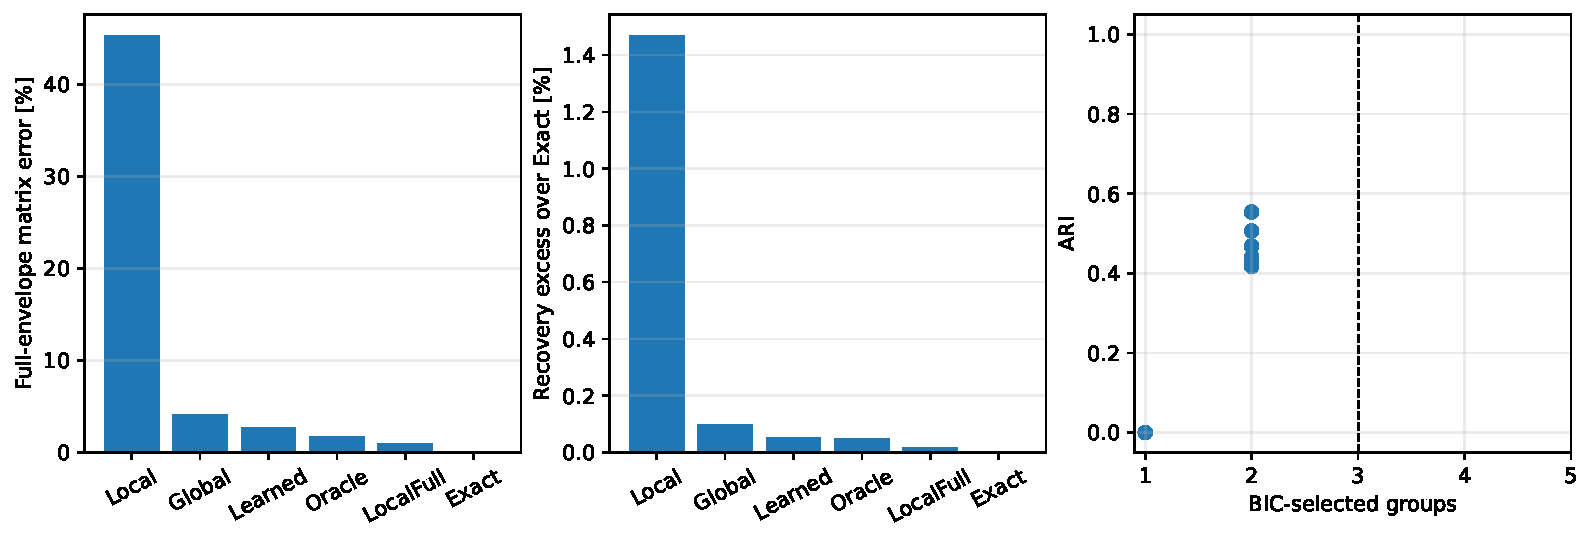
\includegraphics[width=0.98\linewidth]{../results/figures/experiment_10d_learned_groups.pdf}
\caption{Experiment 10D model error, recovery excess over ExactLPV, and the
BIC-selected group count versus adjusted Rand index (ARI).}
\label{fig:experiment10d}
\end{figure}

\paragraph{Result.}
The primary label-free sharing gate passes. LearnedCluster reduces matrix error
by 94.06\% relative to Local and improves nonlinear recovery by 1.398\%; both
intervals are bounded away from zero and all ten fleets are feasible. It also
improves matrix error by 34.27\% relative to Global. The associated recovery
gain over Global is only 0.046\%, although its interval is positive, so this
comparison should be interpreted as near-equivalent closed-loop behavior with
substantially better model fidelity.

Learned grouping does not reach the oracle identification accuracy. Its matrix
error is 62.25\% higher than OracleFamily, although their recovery is
statistically indistinguishable. Relative to Local, LearnedCluster retains
97.7\% of the matrix-error reduction delivered by OracleFamily and essentially
all of its recovery reduction. LocalFull remains the most accurate finite-data
reference because it gives every client an equal total transition budget over
the complete speed envelope; it is a data-acquisition upper reference rather
than a cold-start competitor.

\paragraph{What the groups mean.}
BIC selects two groups in nine fleets and one group in the remaining fleet. It
never selects the simulator's three-family count, and mean ARI is 0.418. In the
nine two-group solutions, the handling and heavy families occupy opposite
groups, while nominal clients are merged with or split between them. This is
not a failed family classifier. It shows that the penalized prediction task
supports fewer shared backbones than the data generator has physical labels.
The distinction is important: Experiment 10D learns a compact compatibility
partition for LPV estimation, not vehicle taxonomy.

\paragraph{Decision and limitation.}
The experiment removes oracle labels from the positive complementary-sharing
result and supports moving to a federated implementation of latent compatible
backbone learning. It does not yet demonstrate federation: the current
alternating fit is centralized and accesses clients' matrix observations.
Moreover, block stratification uses simulator labels to balance the evaluation,
although labels are absent from the estimator. A final federated experiment
must reproduce the alternating sufficient-statistic updates, account for
candidate-count selection and communication, and test non-stratified coverage
or partial participation. Personalization need not be part of that central
claim; Experiment 10C already showed no closed-loop benefit for it.

\paragraph{Reproducibility.}
The configuration and implementation are in
\path{code/config/experiment_10d.json} and
\path{code/experiments/experiment_10d_learned_compatible_groups.py}. Per-fleet
client records, candidate BIC scores, assignments, aggregate summaries, paired
bootstrap comparisons, and provenance hashes are stored under
\path{results/tables}.
